\section{Introduction}
\label{sec:intro}

\subsection{Présentation des laboratoires}
\label{sub:labo}

\subsubsection{AIST-JRL}
\label{sub:JRL}


\includegraphics[width=2.0cm]{images/Logo-AIST-only.jpg}
L'AIST --\emph{Advanced Industrial Science and Technology}-- est un complexe scientifique de recherche situé à Tsukuba dans la préfecture d'Ibaraki au nord-est de Tokyo. Les thèmes de recherches sont variés : biologie, environnement, matériaux, santé, énergies mais également robotique. C'est le laboratoire franco-japonais du JRL --\emph{Joint Robotics Laboratory}-- qui s'occupe de cette branche. Il se spécialise dans la robotique humanoïde en utilisant principalement les robots du projet HRP\footnote{Humanoid Robotics Project} comme le HRP-2 sur lequel j'ai travaillé, mais également les générations plus récentes, le HRP-3 et HRP-4.

La partie française du JRL est composée de trois membres permanents : \olivier, \eiichi et \abder le directeur. Ils sont responsables des différents stagiaires et doctorants qui viennent y réaliser leurs recherches. En comptant les stagiaires, le JRL regroupe donc une petite communauté d'une quinzaine de français.

\subsubsection{LAAS-CNRS}
\label{sub:LAAS}


\includegraphics[width=2.0cm]{images/Logo-LAAS-CNRS.jpg}
Le LAAS --\emph{Laboratoire d'Analyse et d'Architecture des Systèmes}-- est un laboratoire scientifique de recherche du CNRS créé en 1968. Environ 600 personnes y travaillent quotidiennement, réparti en différents groupes de recherche autour de quatre thèmes principaux (Micro et Nanosystèmes, Modélisation et Commande des Systèmes, Systèmes Informatiques Critiques, Robotique et Intelligence Artificielle). J'ai été affecté au groupe G\textsc{epetto}, constitué d'une quinzaine de personnes qui se concentre sur le mouvement humanoïde. 
Un robot humanoïde, le \textbf{HRP-2 Promet 14} (voir figure~\ref{fig:robots}) est présent au sein du laboratoire, c'est sur celui-ci que j'ai réalisé la quasi-totalité des expériences.

Suite à mon retour en France, j'ai pu y travailler avec les étudiants en thèse dont \nicolas et \thomas qui m'ont énormément aidé et conseillé et avec qui j'ai écrit et soumis plusieurs articles. 


\subsection{Robotique humano\"\i de}
\label{sub:robotique}

La robotique humanoïde est un thème de recherche de plus en plus développé. En effet, les domaines d'applications ne sont pas encore nombreux, mais on y retrouve déjà les robots ludiques comme le robot N\textsc{ao} (voir figure~\ref{fig:robots}) de la société française A\textsc{ldebaran} Robotics qui est un jouet de haute technologie.
Il est également souvent utilisé pour la recherche dans les universités, car il est abordable financièrement et assez facilement utilisable.
Un autre centre d'intérêt de la robotique humanoïde est l'assitance à domicile, comme le spécifie le projet R\textsc{omeo} initié par la même entreprise : il sera destiné à l'assistance aux personnes en situation de perte d'autonomie due à leur âge ou à un handicap.

\begin{figure}[h]
\begin{center}
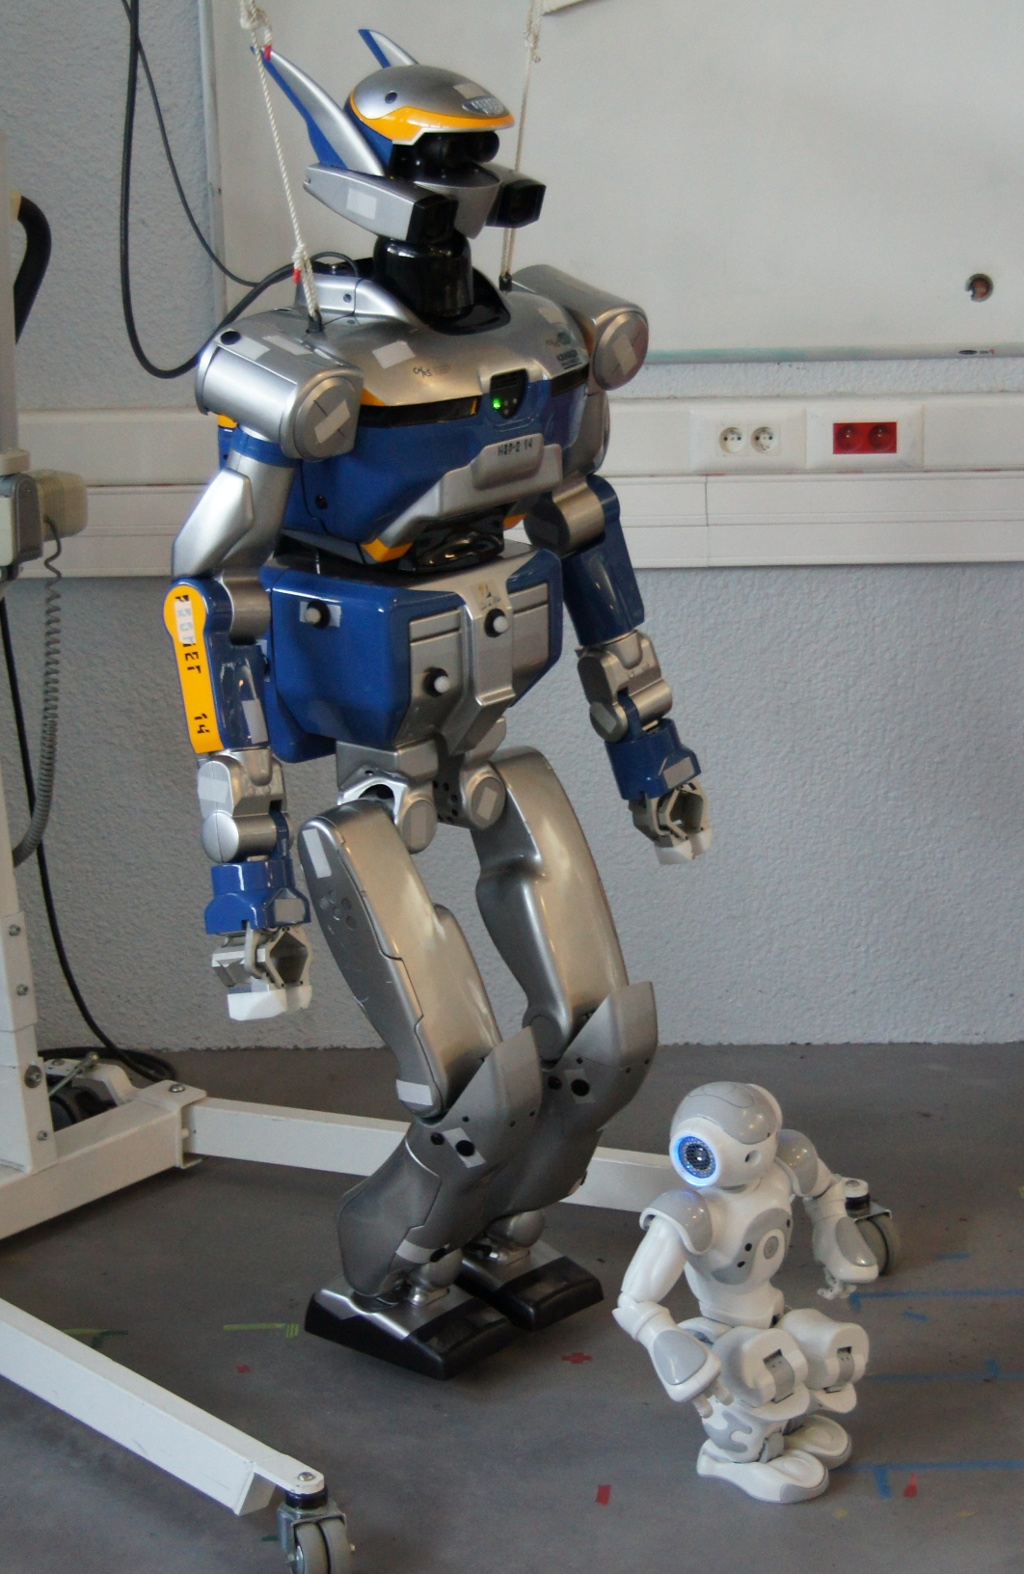
\includegraphics[width=7.0cm]{images/robots.jpg}
\caption{Deux robots humanoïdes : HRP-2 (gauche) de K\textsc{awada} I\textsc{ndustries} et N\textsc{ao} (droite) de A\textsc{ldebaran} R\textsc{obotics}}
\label{fig:robots}
\end{center}
\end{figure}

Cependant la robotique humanoïde n'en est qu'à ses débuts. Effectivement, malgré les différents algorithmes proposés permettant à un robot de naviguer dans un espace donné, il est encore difficile de faire marcher correctement un robot dans un environnement adapté à l'être humain. 
Afin de pouvoir se déplacer il doit être capable de marcher dans des environnements très contraints avec de nombreux obstacles. 
Pour l'instant la plupart des algorithmes qui permettent l'évitement d'obstacles utilisent le principe suivant : la projection du robot sur le sol ne doit pas entrer dans celle des obstacles \cite{Chestnutt:ICRA:2005}. On parlera donc d'évitement de collisions en 2D. 
Dès que l'on passe sur des détections de collisions en 3D, en tenant compte de la géométrie réelle du robot et celle des obstacles, les algorithmes deviennent alors relativement lents principalement à cause de la puissance de calcul nécessaire pour les tests de collisions en 3D. Certains algorithmes se limitent donc à des formes géométriques simples~\cite{gutmann:ijrr:2008}.

%D'autre part trouver une trajectoire optimale pour un robot revient souvent à rechercher le plus cours chemin dans un graphe. Dans la section \ref{sub:RRT} sera expliqué le choix de l'algoritme RRT pour trouver un chemin faisable. 
Mon travail principal durant ce stage a été d'utiliser les méthodes développées par \nicolas pour de la planification, afin de les transposer sur des applications de replanification en temps réel. J'utiliserai donc souvent comme référence son article \cite{perrin:TRO:2011} qui m'a servi de base tout au long de ce stage, et auquel j'ai participé.

Récemment la navigation 3D pour les robots humanoïdes \cite{Chestnutt:IROS:2009,Chestnutt:MPHR:2010} a été mise en place mais elle ne concerne que des environnements statiques. Nous avons considéré des obstacles 3D afin de gérer les évitements de collisions avec le corps du robot de manière précise selon une méthode fondée sur la planification de mouvements rapides utilisant des volumes balayés~\cite{perrin:TRO:2011}.
\vspace{4mm}

Ce rapport suivra l'organisation suivante : dans la section \ref{sec:planif} nous verrons comment est mis en place le processus de planification de pas. Le contrôle du robot sera présenté dans la section \ref{sec:control} puis les expériences et leurs résultats dans la section \ref{sec:exp}. Une conclusion sur les travaux effectués et restants terminera ce rapport.

%for example restricting the obstacles to 2D shapes \cite{Chestnutt:ICRA:2005} or simple geometries \cite{gutmann:ijrr:2008}.
%recently interactive 3D navigation by humanoid
%\cite{Chestnutt:IROS:2009}\cite{Chestnutt:MPHR:2010} has been reported, but it is for static environments.
%In this paper, we consider 3D moving obstacles and handle the collision avoidance with the legs in an accurate way, based on fast motion planning with precomputed dense swept volumes \cite{perrin:TRO:2011}, whereas only sparse finite footsteps are considered in \cite{Chestnutt:IROS:2009}\cite{Chestnutt:MPHR:2010}. 
